% filename: Solution_IO.tex
\documentclass[10pt]{article}
\include{PhysNote}
%\usepackage{srcltx}

\usepackage{graphicx} % to insert images
\usepackage{grffile}  % to allow filenames with multiple dots (to get rid of "Unknown graphics extension" error)

\title{Solution IO (Input and Output)}
\subtitle{for LeetCode problem 210 Course Schedule II}
\author{Andrew Forrester}
\date{}
%\date{2019 June 22}
\setcounter{section}{0}

\begin{document}
\maketitle


\section*{Instance 1}

\squishlist
  \item \parbox{40pt}{Input:}  \url{2, [[1,0]]}
\squishend
\begin{figure}[h!]
  \hspace{50pt}
  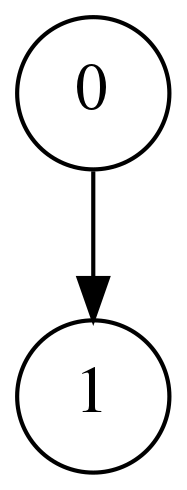
\includegraphics[width=20pt]{Input/Graph_1.gv.png}
\end{figure}

\squishlist
  \item \parbox{40pt}{Output:} \url{[0, 1]}
\squishend
\begin{figure}[h!]
  \hspace{50pt}
  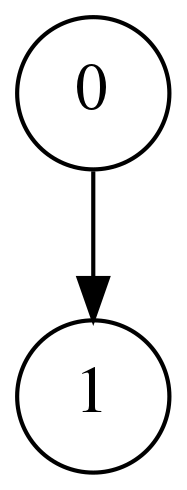
\includegraphics[width=20pt]{Input/Graph_1.gv.png}
\end{figure}


\section*{Instance 2}

\squishlist
  \item \parbox{40pt}{Input:}  \url{2, [[1,0],[0,1]]}
\squishend
\begin{figure}[h!]
  \hspace{50pt}
  
\includegraphics[width=20pt]{Input/Graph_2a.gv.png}
  \hspace{50pt}
  \raisebox{25pt}{or}
  \hspace{50pt}
  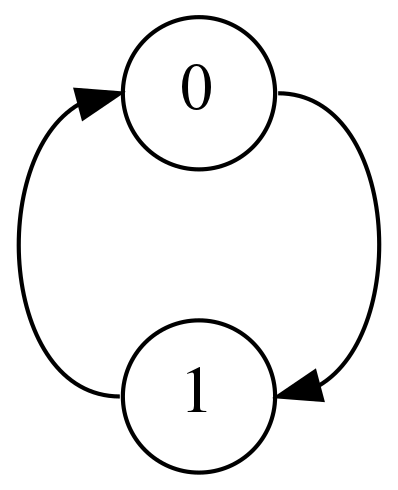
\includegraphics[width=40pt]{Input/Graph_2b.gv.png}
\end{figure}

\squishlist
  \item \parbox{40pt}{Output:} \url{[]}
\squishend


\section*{Instance 3}

\squishlist
  \item \parbox{40pt}{Input:}  \url{4, [[1,0],[2,1],[3,2],[1,3]]}
\squishend
\begin{figure}[h!]
  \hspace{50pt}
  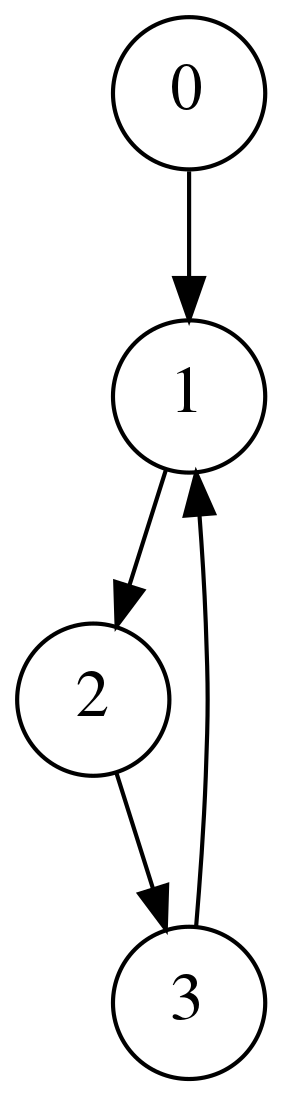
\includegraphics[width=30pt]{Input/Graph_3a.gv.png}
  \hspace{50pt}
  \raisebox{50pt}{or}
  \hspace{50pt}
  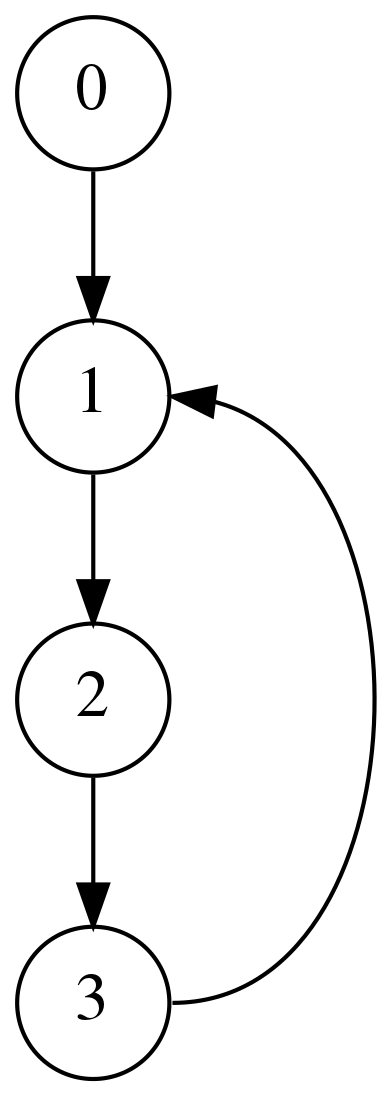
\includegraphics[width=40pt]{Input/Graph_3b.gv.png}
  \hspace{50pt}
  \raisebox{50pt}{or}
  \hspace{50pt}
  \raisebox{0.33\height}{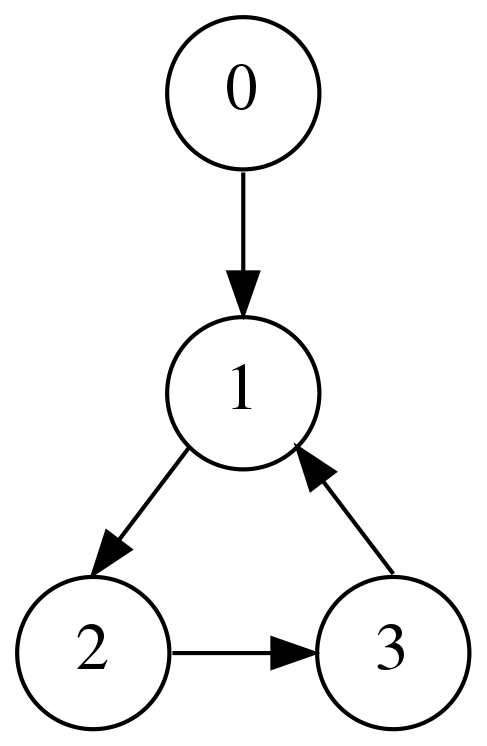
\includegraphics[width=50pt]{Input/Graph_3c.gv.png}}
\end{figure}

\squishlist
  \item \parbox{40pt}{Output:} \url{[]}
\squishend


\section*{Instance 4}

\squishlist
  \item \parbox{40pt}{Input:}  \url{6, [[1,0],[3,2],[5,2],[1,4],[1,5]]}
\squishend
\begin{figure}[h!]
  \hspace{50pt}
  \raisebox{0.6\height}{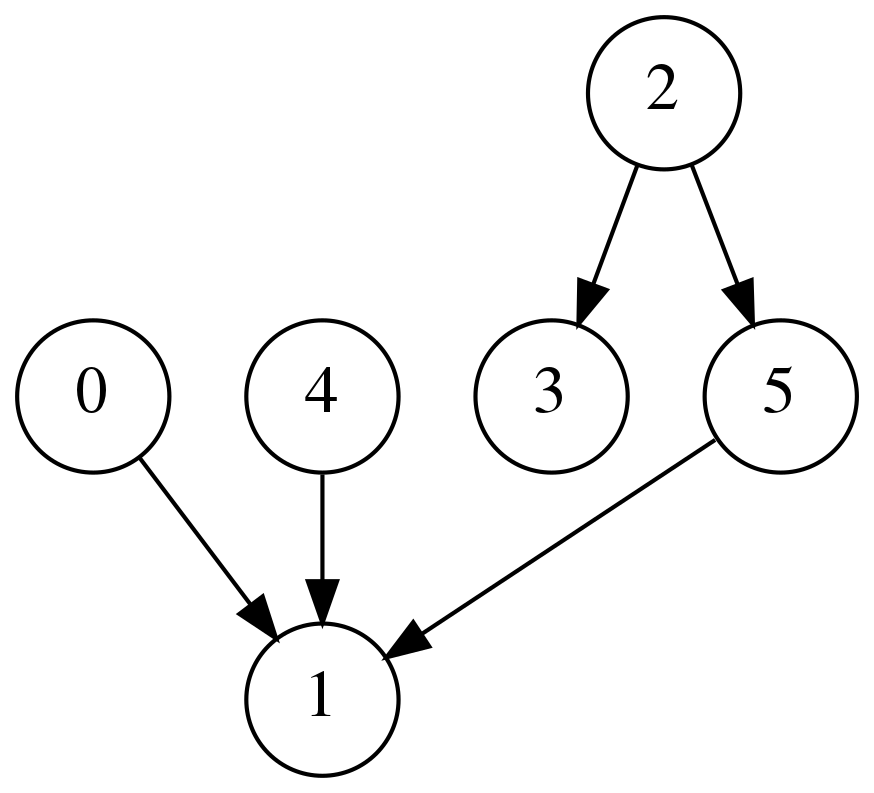
\includegraphics[width=90pt]{Input/Graph_4a.gv.png}}
  \hspace{50pt}
  \raisebox{90pt}{or}
  \hspace{50pt}
  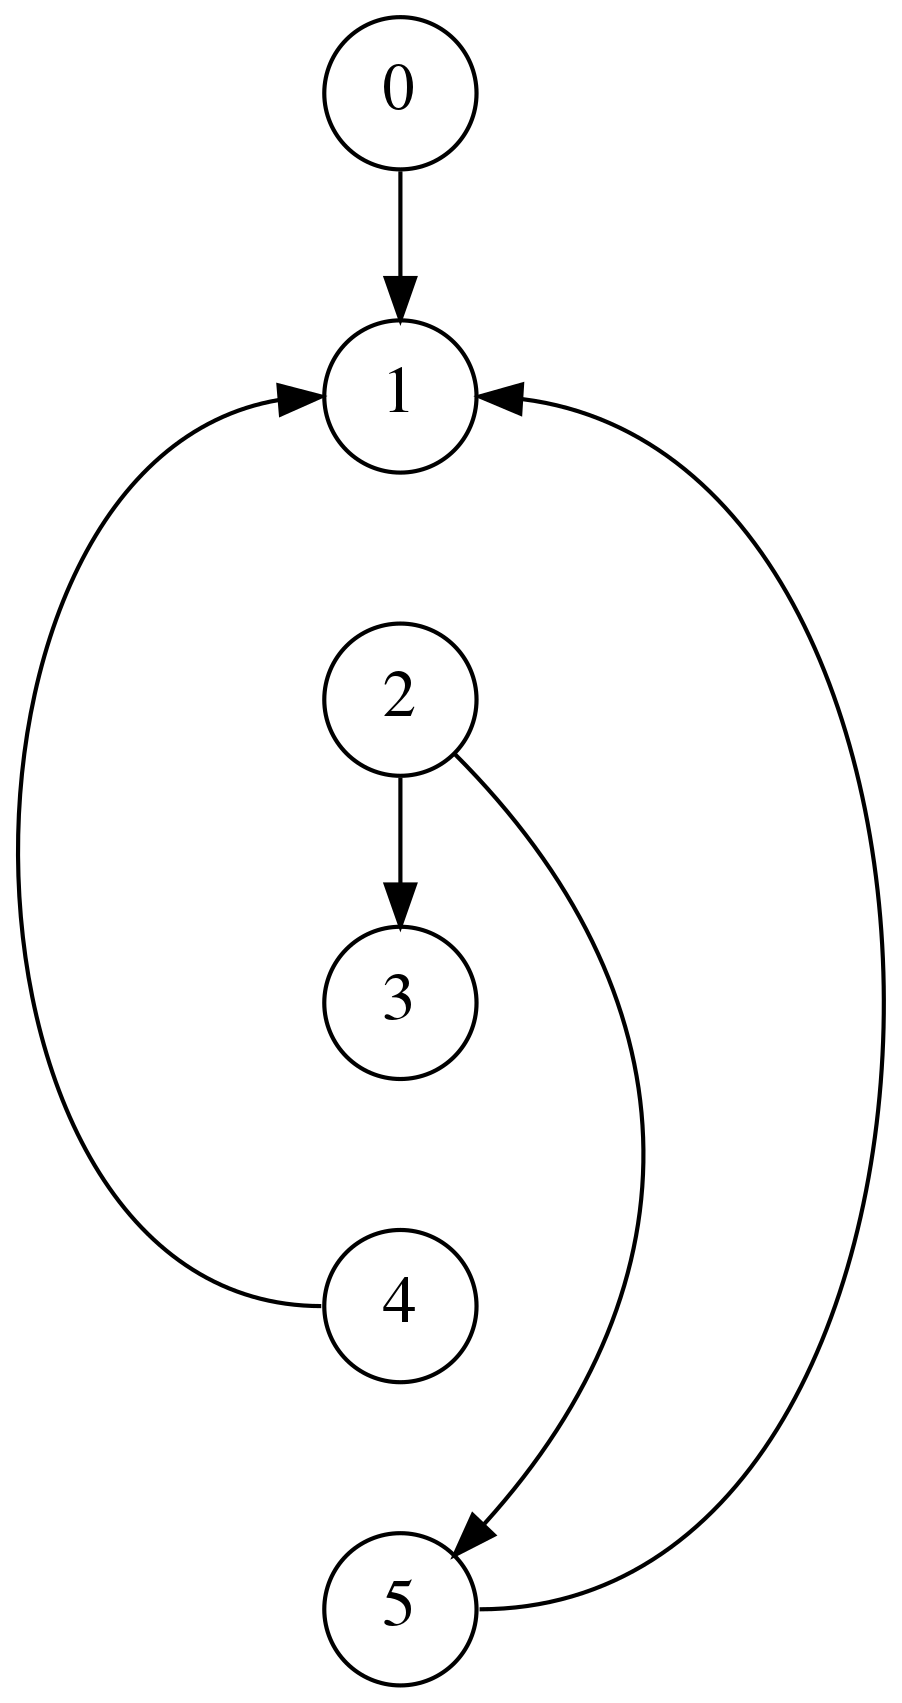
\includegraphics[width=90pt]{Input/Graph_4b.gv.png}
\end{figure}

\squishlist
  \item \parbox{40pt}{Output:} \url{[0, 2, 4, 3, 5, 1]}
\squishend
\begin{figure}[h!]
  \hspace{50pt}
  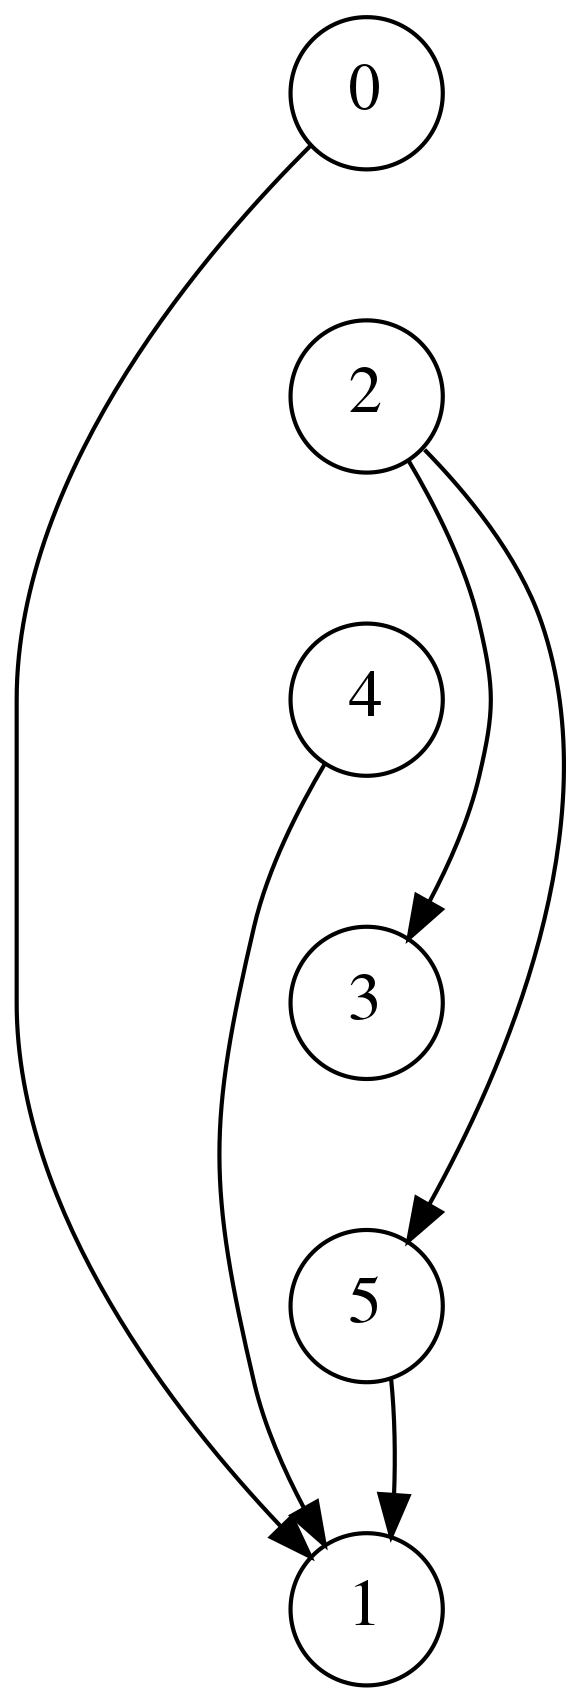
\includegraphics[width=60pt]{Output/Graph_4_soln.gv.png}
\end{figure}


\newpage

\section*{Instance 5}

\squishlist
  \item \parbox{40pt}{Input:}  \url{6, [[1,0],[5,2],[3,5],[4,3],[2,4]]}
\squishend
\begin{figure}[h!]
  \hspace{50pt}
  \raisebox{0.25\height}{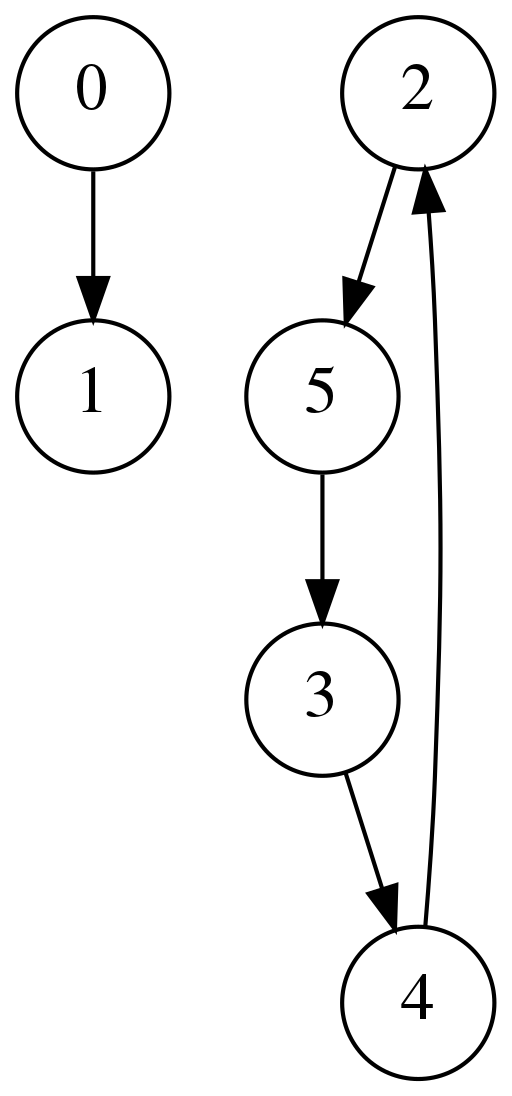
\includegraphics[width=55pt]{Input/Graph_5a.gv.png}}
  \hspace{50pt}
  \raisebox{90pt}{or}
  \hspace{50pt}
  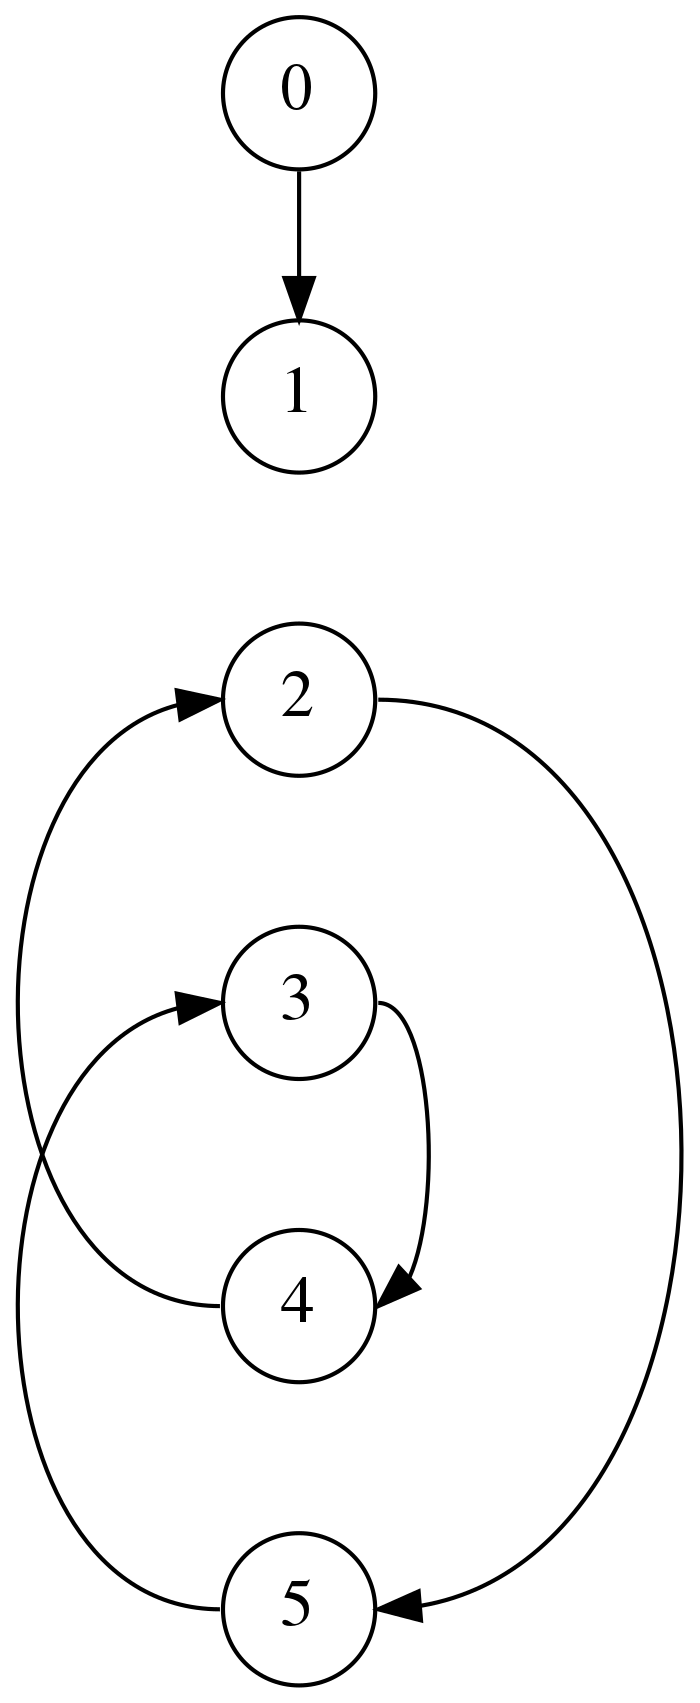
\includegraphics[width=75pt]{Input/Graph_5b.gv.png}
\end{figure}

\squishlist
  \item \parbox{40pt}{Output:} \url{[]}
\squishend


\newpage

\section*{Instance 6}

\squishlist
  \item \parbox{40pt}{Input:}  \url{6, [[1,0],[2,0],[3,0],[4,0],[5,0],[2,1],[5,4]]}
\squishend
\begin{figure}[h!]
  \hspace{50pt}
  \raisebox{0.5\height}{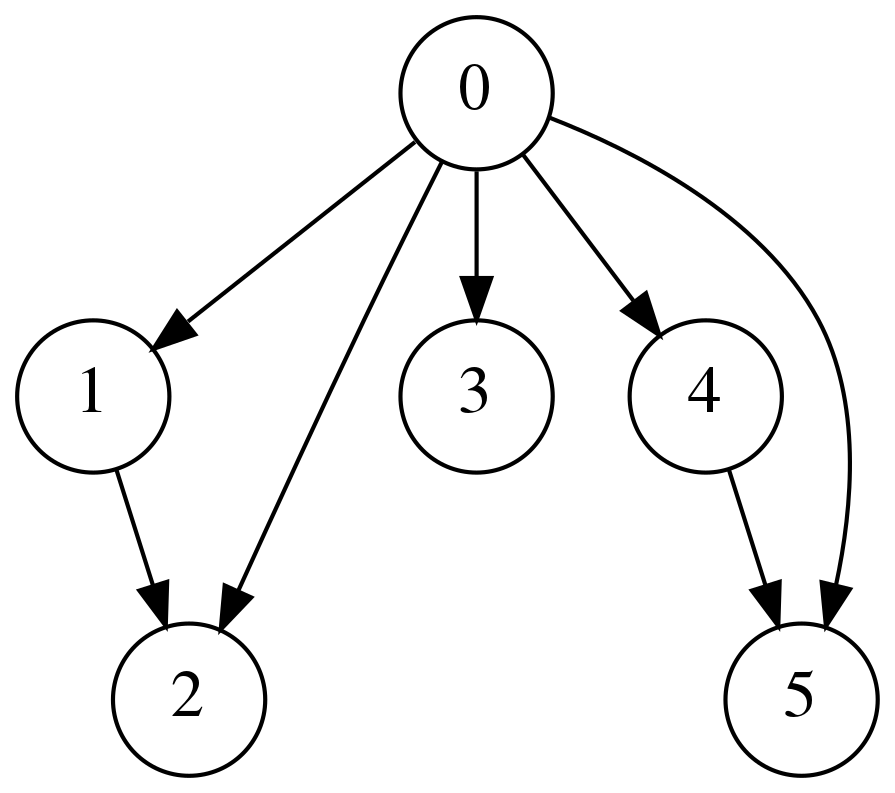
\includegraphics[width=100pt]{Input/Graph_6a.gv.png}}
  \hspace{50pt}
  \raisebox{90pt}{or}
  \hspace{50pt}
  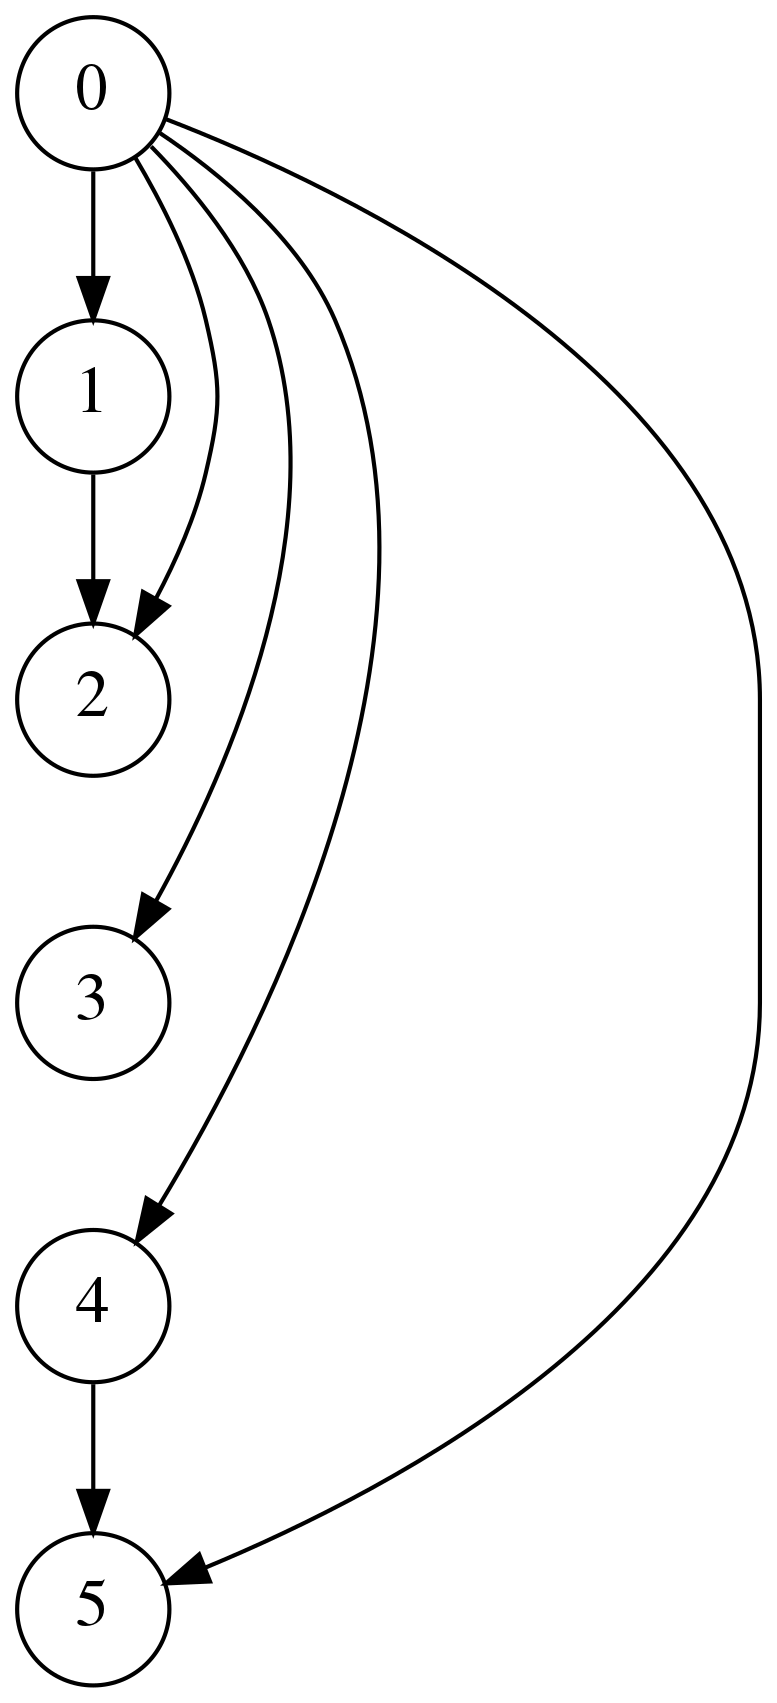
\includegraphics[width=80pt]{Input/Graph_6b.gv.png}
\end{figure}

\squishlist
  \item \parbox{40pt}{Output:} \url{[0, 1, 3, 4, 2, 5]}
\squishend
\begin{figure}[h!]
  \hspace{50pt}
  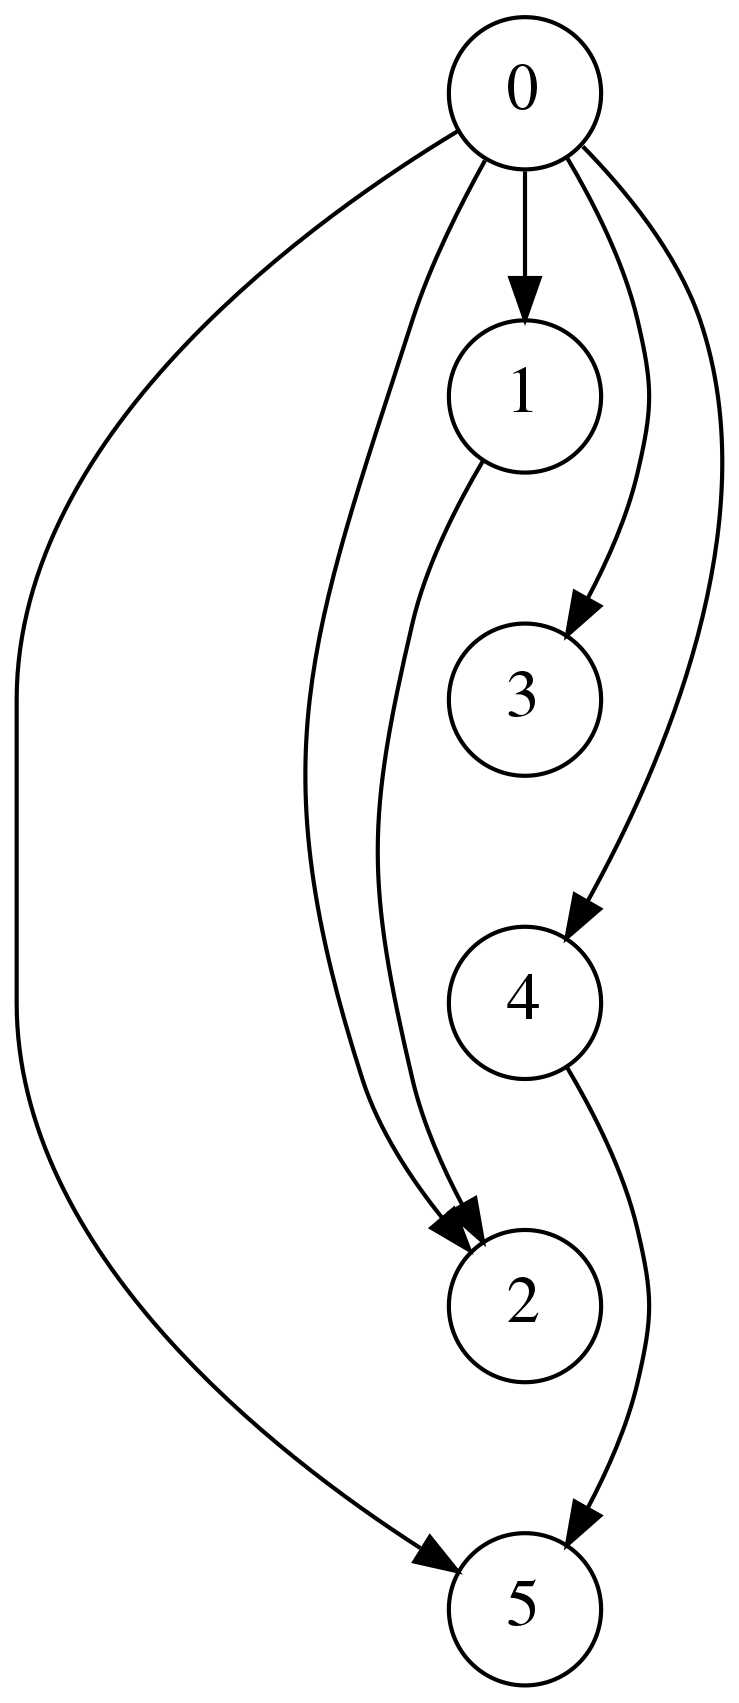
\includegraphics[width=80pt]{Output/Graph_6_soln.gv.png}
\end{figure}


\newpage

\section*{Instance 7}

\squishlist
  \item \parbox{40pt}{Input:}  \url{6, [[1,0],[1,4],[1,5],[3,2],[5,2]]}
\squishend
\begin{figure}[h!]
  \hspace{50pt}
  \raisebox{0.5\height}{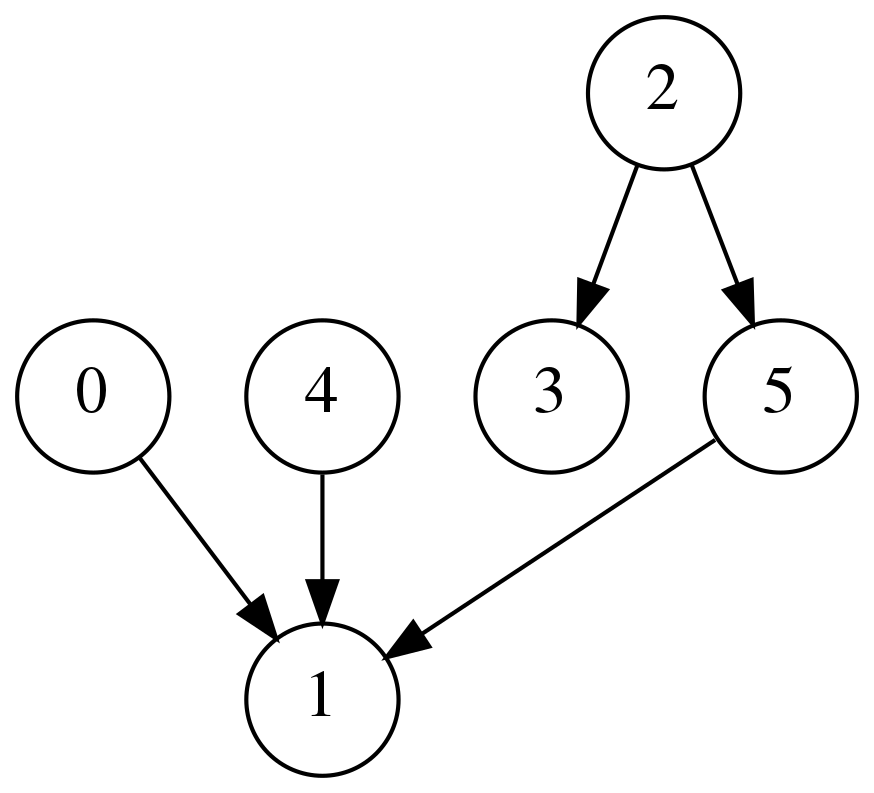
\includegraphics[width=90pt]{Input/Graph_7a.gv.png}}
  \hspace{50pt}
  \raisebox{80pt}{or}
  \hspace{50pt}
  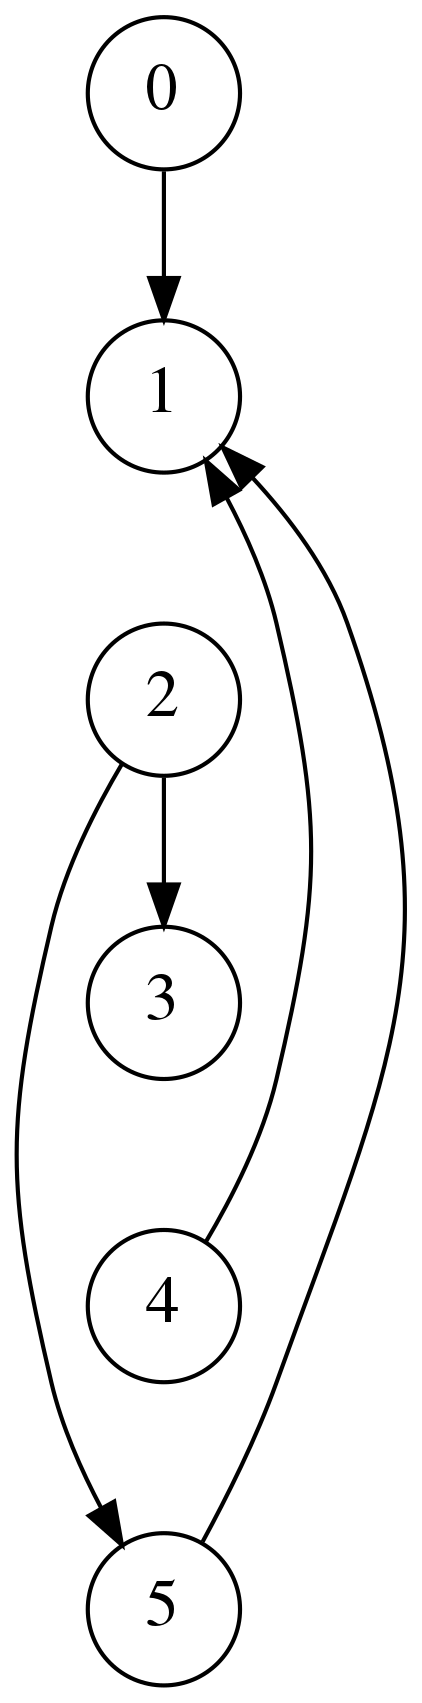
\includegraphics[width=40pt]{Input/Graph_7b.gv.png}
\end{figure}

\squishlist
  \item \parbox{40pt}{Output:} \url{[0, 2, 4, 3, 5, 1]}
\squishend
\begin{figure}[h!]
  \hspace{50pt}
  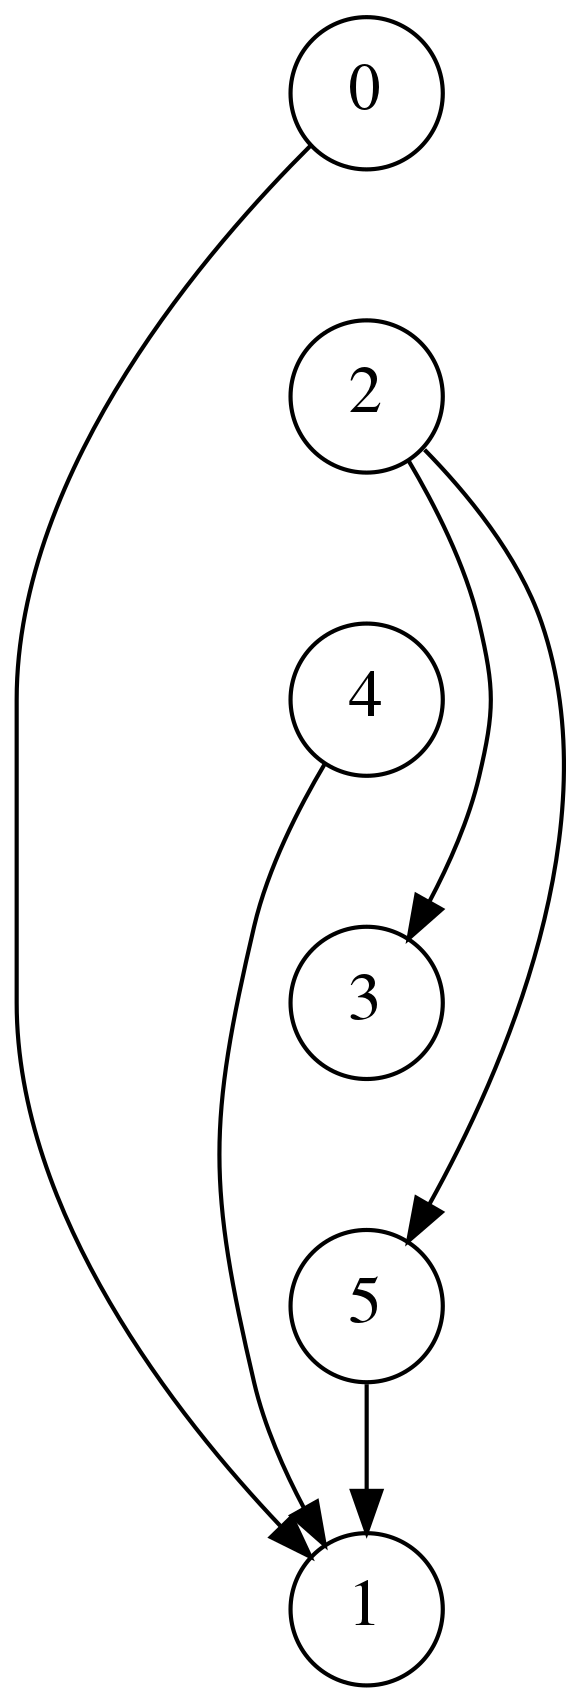
\includegraphics[width=60pt]{Output/Graph_7_soln.gv.png}
\end{figure}


\newpage

\section*{Instance 8}

\squishlist
  \item \parbox{40pt}{Input:}  \url{6, [[2,0],[3,1],[4,2],[5,2],[5,3]]}
\squishend
\begin{figure}[h!]
  \hspace{50pt}
  \raisebox{0.5\height}{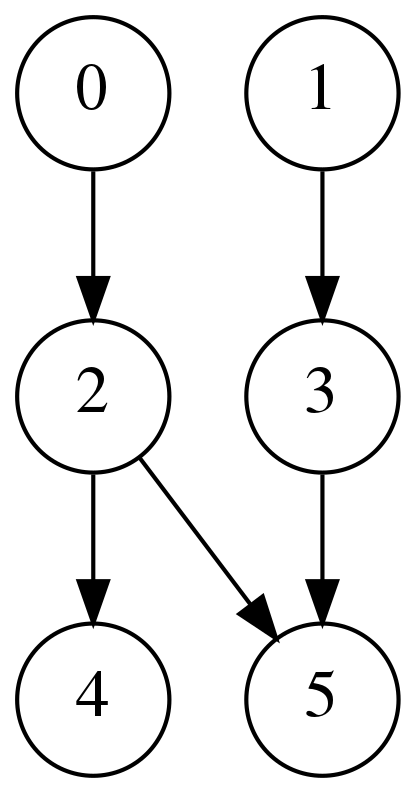
\includegraphics[width=45pt]{Input/Graph_8a.gv.png}}
  \hspace{50pt}
  \raisebox{80pt}{or}
  \hspace{50pt}
  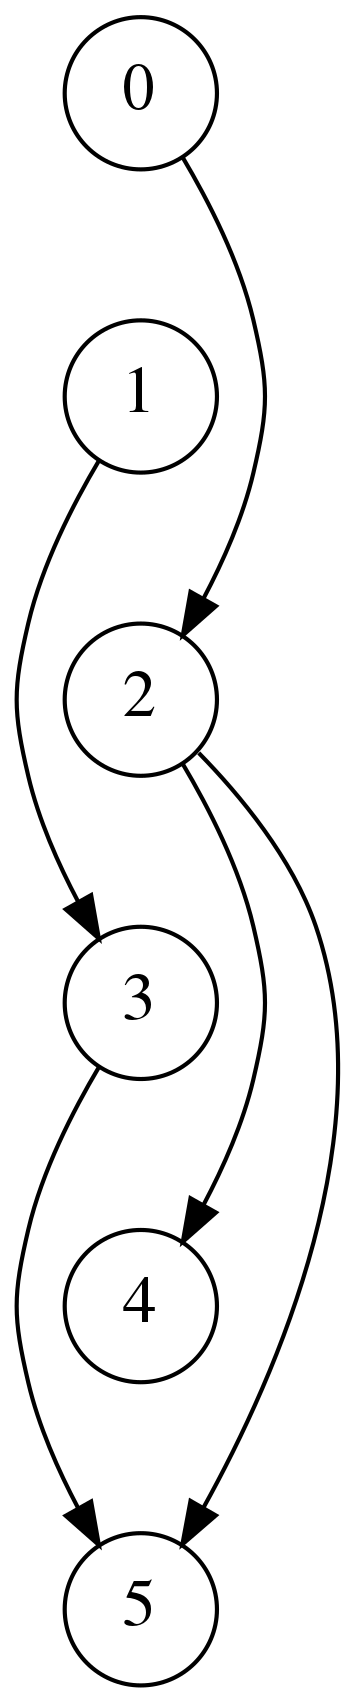
\includegraphics[width=35pt]{Input/Graph_8b.gv.png}
\end{figure}

\squishlist
  \item \parbox{40pt}{Output:} \url{[0, 1, 2, 3, 4, 5]}
\squishend
\begin{figure}[h!]
  \hspace{50pt}
  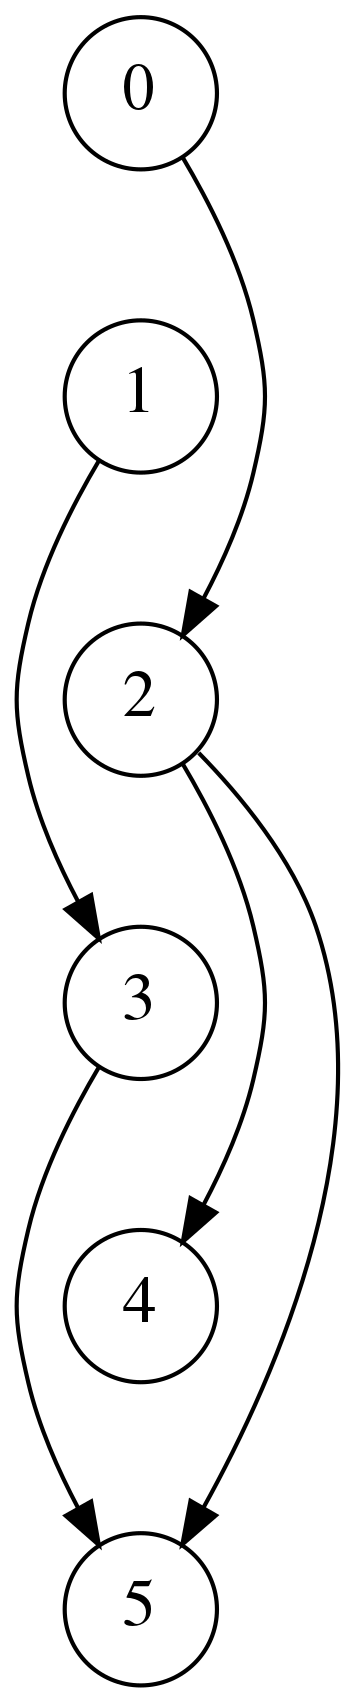
\includegraphics[width=35pt]{Output/Graph_8_soln.gv.png}
\end{figure}


\newpage

\section*{Instance 9}

\squishlist
  \item \parbox{40pt}{Input:}  \url{9, [[2,0],[2,1],[3,0],[3,1],[4,2],[5,3],[6,5],[7,5],[8,4],[8,6],[8,7]]}
\squishend
\begin{figure}[h!]
  \hspace{50pt}
  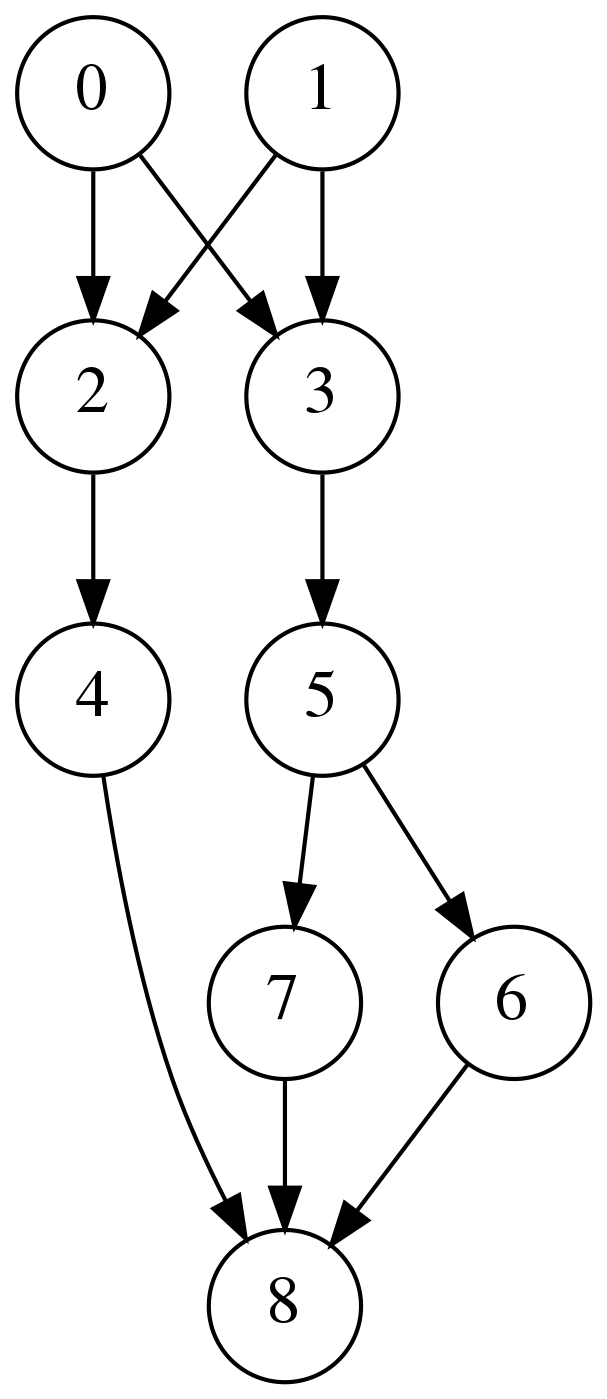
\includegraphics[width=65pt]{Input/Graph_9.gv.png}
\end{figure}

\squishlist
  \item \parbox{40pt}{Output:} \url{[0, 1, 2, 3, 4, 5, 6, 7, 8]}
\squishend
\begin{figure}[h!]
  \hspace{50pt}
  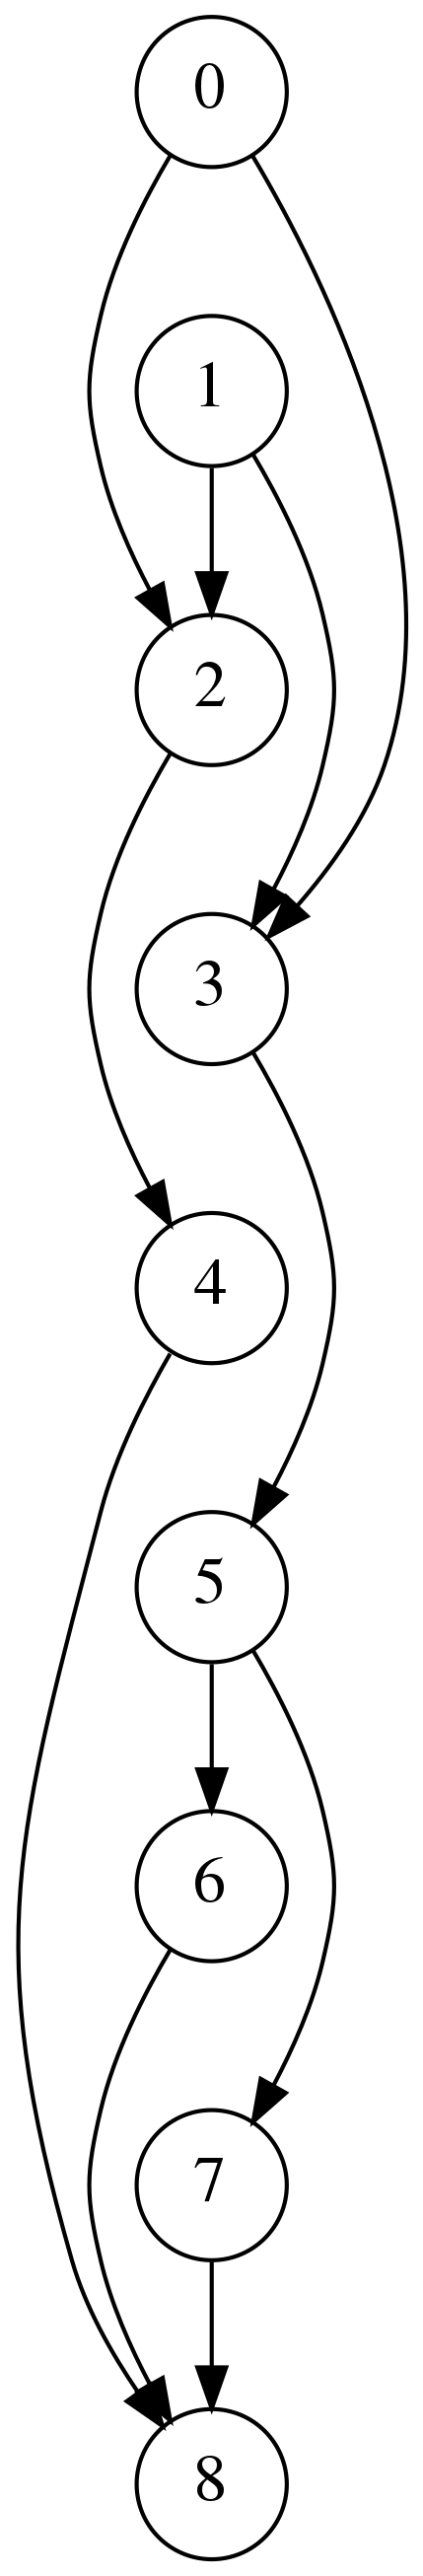
\includegraphics[width=45pt]{Output/Graph_9_soln.gv.png}
\end{figure}



\end{document}
